\documentclass{standalone}
\usepackage{tikz}
\usetikzlibrary{patterns, positioning}
\usepackage[sfdefault]{ClearSans} %% option 'sfdefault' activates Clear Sans as the default text font
\usepackage[T1]{fontenc}

\begin{document}
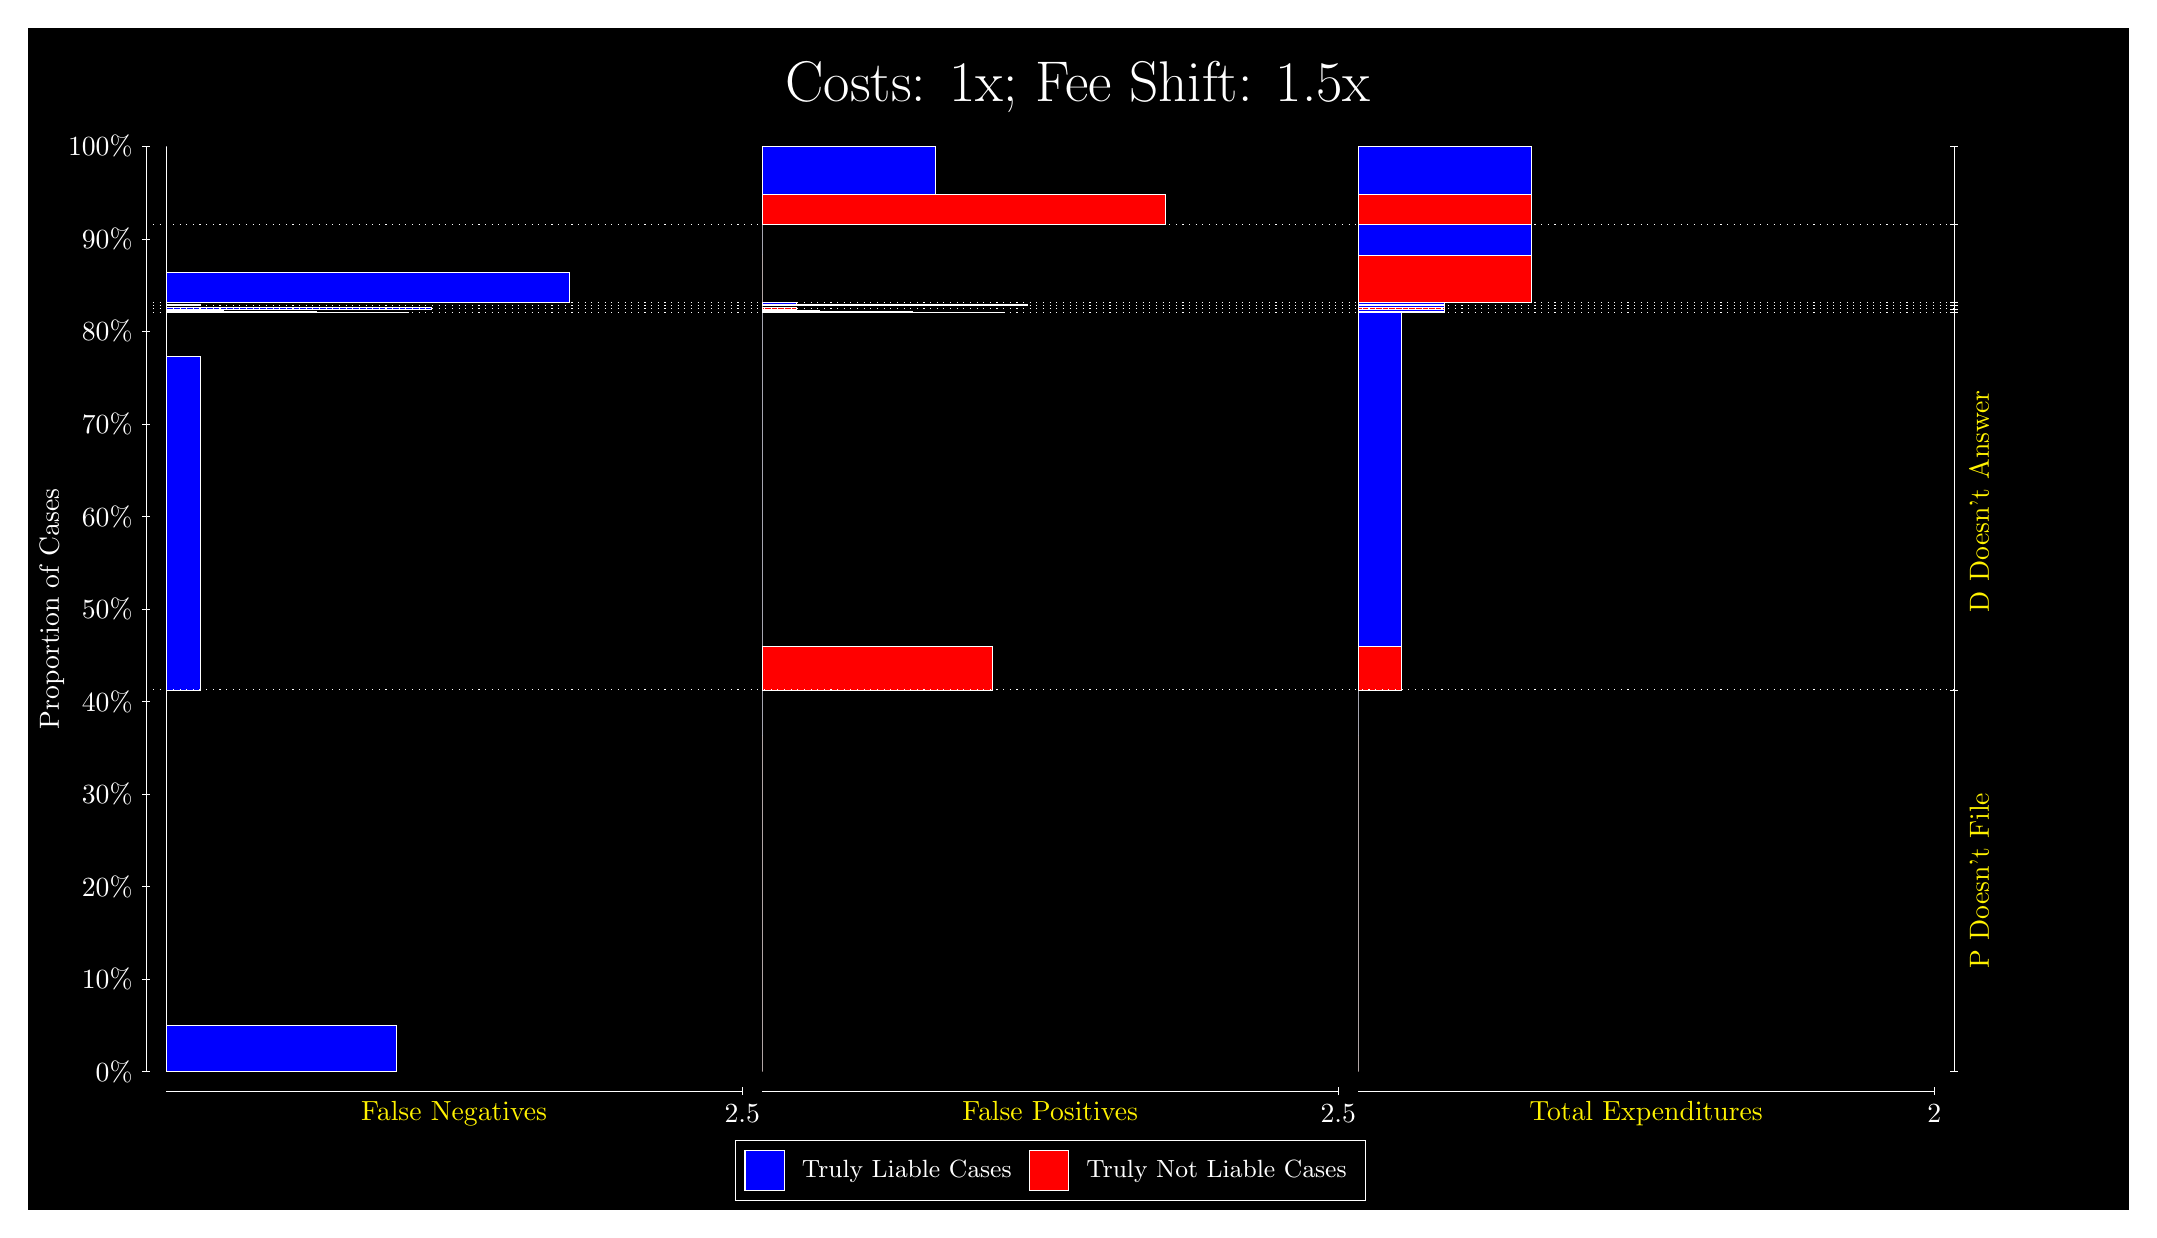
\begin{tikzpicture}
\draw[fill=black] (0,0) rectangle (26.667,15);
\draw[text=white] (0,13.5) rectangle (26.667,15) node[midway] {\huge Costs: 1x; Fee Shift: 1.5x};
\draw[white, very thin] (1.5,1.75) -- (1.5,13.5);
\node[rotate=90, text=white, anchor=center] at (0.3, 7.625) {Proportion of Cases};
\draw[white, very thin] (1.45,1.75) -- (1.55,1.75);
\node[text=white, anchor=east] at (1.45, 1.75) {0\%};
\draw[white, very thin] (1.45,2.925) -- (1.55,2.925);
\node[text=white, anchor=east] at (1.45, 2.925) {10\%};
\draw[white, very thin] (1.45,4.1) -- (1.55,4.1);
\node[text=white, anchor=east] at (1.45, 4.1) {20\%};
\draw[white, very thin] (1.45,5.275) -- (1.55,5.275);
\node[text=white, anchor=east] at (1.45, 5.275) {30\%};
\draw[white, very thin] (1.45,6.45) -- (1.55,6.45);
\node[text=white, anchor=east] at (1.45, 6.45) {40\%};
\draw[white, very thin] (1.45,7.625) -- (1.55,7.625);
\node[text=white, anchor=east] at (1.45, 7.625) {50\%};
\draw[white, very thin] (1.45,8.8) -- (1.55,8.8);
\node[text=white, anchor=east] at (1.45, 8.8) {60\%};
\draw[white, very thin] (1.45,9.975) -- (1.55,9.975);
\node[text=white, anchor=east] at (1.45, 9.975) {70\%};
\draw[white, very thin] (1.45,11.15) -- (1.55,11.15);
\node[text=white, anchor=east] at (1.45, 11.15) {80\%};
\draw[white, very thin] (1.45,12.325) -- (1.55,12.325);
\node[text=white, anchor=east] at (1.45, 12.325) {90\%};
\draw[white, very thin] (1.45,13.5) -- (1.55,13.5);
\node[text=white, anchor=east] at (1.45, 13.5) {100\%};

\draw[white, very thin] (24.457,1.75) -- (24.457,13.5);
\draw[white, very thin] (24.407,1.75) -- (24.507,1.75);
\node[anchor=west] at (24.407, 1.75) {};
\draw[white, very thin] (24.407,6.5975) -- (24.507,6.5975);
\node[anchor=west] at (24.407, 6.5975) {};
\draw[white, very thin] (24.407,11.39) -- (24.507,11.39);
\node[anchor=west] at (24.407, 11.39) {};
\draw[white, very thin] (24.407,11.436) -- (24.507,11.436);
\node[anchor=west] at (24.407, 11.436) {};
\draw[white, very thin] (24.407,11.476) -- (24.507,11.476);
\node[anchor=west] at (24.407, 11.476) {};
\draw[white, very thin] (24.407,11.516) -- (24.507,11.516);
\node[anchor=west] at (24.407, 11.516) {};
\draw[white, very thin] (24.407,12.508) -- (24.507,12.508);
\node[anchor=west] at (24.407, 12.508) {};
\draw[white, very thin] (24.407,13.5) -- (24.507,13.5);
\node[anchor=west] at (24.407, 13.5) {};

\draw[white, very thin, fill=blue] (1.75,1.75) rectangle (4.6775,2.3331);
\draw[white, very thin, fill=red] (1.75,2.3331) rectangle (1.75,6.5975);
\draw[white, very thin, fill=blue] (1.75,6.5975) rectangle (2.1891,10.835);
\draw[white, very thin, fill=red] (1.75,10.835) rectangle (1.75,11.39);
\draw[white, very thin, fill=blue] (1.75,11.39) rectangle (4.8239,11.393);
\draw[white, very thin, fill=blue] (1.75,11.393) rectangle (4.5312,11.394);
\draw[white, very thin, fill=blue] (1.75,11.394) rectangle (4.2384,11.395);
\draw[white, very thin, fill=blue] (1.75,11.395) rectangle (3.9457,11.396);
\draw[white, very thin, fill=blue] (1.75,11.396) rectangle (3.6529,11.407);
\draw[white, very thin, fill=blue] (1.75,11.407) rectangle (3.3602,11.407);
\draw[white, very thin, fill=blue] (1.75,11.407) rectangle (3.0674,11.409);
\draw[white, very thin, fill=blue] (1.75,11.409) rectangle (2.7746,11.41);
\draw[white, very thin, fill=blue] (1.75,11.41) rectangle (2.4819,11.413);
\draw[white, very thin, fill=red] (1.75,11.413) rectangle (1.75,11.436);
\draw[white, very thin, fill=blue] (1.75,11.436) rectangle (5.1167,11.453);
\draw[white, very thin, fill=red] (1.75,11.453) rectangle (1.75,11.476);
\draw[white, very thin, fill=blue] (1.75,11.476) rectangle (2.1891,11.499);
\draw[white, very thin, fill=red] (1.75,11.499) rectangle (1.75,11.516);
\draw[white, very thin, fill=blue] (1.75,11.516) rectangle (6.8732,11.903);
\draw[white, very thin, fill=red] (1.75,11.903) rectangle (1.75,12.508);
\draw[white, very thin, fill=red] (1.75,12.508) rectangle (1.75,12.895);
\draw[white, very thin, fill=blue] (1.75,12.895) rectangle (1.75,13.5);
\draw[white, very thin, fill=red] (9.3189,1.75) rectangle (9.3189,6.0143);
\draw[white, very thin, fill=blue] (9.3189,6.0143) rectangle (9.3189,6.5975);
\draw[white, very thin, fill=red] (9.3189,6.5975) rectangle (12.246,7.1533);
\draw[white, very thin, fill=blue] (9.3189,7.1533) rectangle (9.3189,11.39);
\draw[white, very thin, fill=red] (9.3189,11.39) rectangle (12.393,11.393);
\draw[white, very thin, fill=red] (9.3189,11.393) rectangle (12.1,11.394);
\draw[white, very thin, fill=red] (9.3189,11.394) rectangle (11.807,11.395);
\draw[white, very thin, fill=red] (9.3189,11.395) rectangle (11.515,11.395);
\draw[white, very thin, fill=red] (9.3189,11.395) rectangle (11.222,11.407);
\draw[white, very thin, fill=red] (9.3189,11.407) rectangle (10.929,11.407);
\draw[white, very thin, fill=red] (9.3189,11.407) rectangle (10.929,11.407);
\draw[white, very thin, fill=red] (9.3189,11.407) rectangle (10.636,11.409);
\draw[white, very thin, fill=red] (9.3189,11.409) rectangle (10.344,11.41);
\draw[white, very thin, fill=red] (9.3189,11.41) rectangle (10.051,11.413);
\draw[white, very thin, fill=blue] (9.3189,11.413) rectangle (9.4652,11.416);
\draw[white, very thin, fill=blue] (9.3189,11.416) rectangle (9.3189,11.436);
\draw[white, very thin, fill=red] (9.3189,11.436) rectangle (9.758,11.458);
\draw[white, very thin, fill=blue] (9.3189,11.458) rectangle (9.3189,11.476);
\draw[white, very thin, fill=red] (9.3189,11.476) rectangle (12.686,11.493);
\draw[white, very thin, fill=blue] (9.3189,11.493) rectangle (9.758,11.516);
\draw[white, very thin, fill=red] (9.3189,11.516) rectangle (9.3189,12.121);
\draw[white, very thin, fill=blue] (9.3189,12.121) rectangle (9.3189,12.508);
\draw[white, very thin, fill=red] (9.3189,12.508) rectangle (14.442,12.895);
\draw[white, very thin, fill=blue] (9.3189,12.895) rectangle (11.515,13.5);
\draw[white, very thin, fill=red] (16.888,1.75) rectangle (16.888,6.0143);
\draw[white, very thin, fill=blue] (16.888,6.0143) rectangle (16.888,6.5975);
\draw[white, very thin, fill=red] (16.888,6.5975) rectangle (17.437,7.1533);
\draw[white, very thin, fill=blue] (16.888,7.1533) rectangle (17.437,11.39);
\draw[white, very thin, fill=red] (16.888,11.39) rectangle (17.986,11.407);
\draw[white, very thin, fill=blue] (16.888,11.407) rectangle (17.986,11.425);
\draw[white, very thin, fill=red] (16.888,11.425) rectangle (17.986,11.428);
\draw[white, very thin, fill=blue] (16.888,11.428) rectangle (17.986,11.43);
\draw[white, very thin, fill=red] (16.888,11.43) rectangle (17.986,11.433);
\draw[white, very thin, fill=blue] (16.888,11.433) rectangle (17.986,11.436);
\draw[white, very thin, fill=red] (16.888,11.436) rectangle (17.986,11.458);
\draw[white, very thin, fill=blue] (16.888,11.458) rectangle (17.986,11.476);
\draw[white, very thin, fill=red] (16.888,11.476) rectangle (17.986,11.493);
\draw[white, very thin, fill=blue] (16.888,11.493) rectangle (17.986,11.516);
\draw[white, very thin, fill=red] (16.888,11.516) rectangle (19.083,12.121);
\draw[white, very thin, fill=blue] (16.888,12.121) rectangle (19.083,12.508);
\draw[white, very thin, fill=red] (16.888,12.508) rectangle (19.083,12.895);
\draw[white, very thin, fill=blue] (16.888,12.895) rectangle (19.083,13.5);
\draw[white, dotted] (1.5,6.5975) -- (24.457,6.5975);
\draw[white, dotted] (1.5,11.39) -- (24.457,11.39);
\draw[white, dotted] (1.5,11.436) -- (24.457,11.436);
\draw[white, dotted] (1.5,11.476) -- (24.457,11.476);
\draw[white, dotted] (1.5,11.516) -- (24.457,11.516);
\draw[white, dotted] (1.5,12.508) -- (24.457,12.508);
\draw[white, very thin] (1.75,1.5) -- (9.0689,1.5);
\node[text=yellow, anchor=north] at (5.4094, 1.5) {False Negatives};
\draw[white, very thin] (9.0689,1.45) -- (9.0689,1.55);
\node[text=white, anchor=north] at (9.0689, 1.45) {2.5};

\draw[white, very thin] (9.3189,1.5) -- (16.638,1.5);
\node[text=yellow, anchor=north] at (12.978, 1.5) {False Positives};
\draw[white, very thin] (16.638,1.45) -- (16.638,1.55);
\node[text=white, anchor=north] at (16.638, 1.45) {2.5};

\draw[white, very thin] (16.888,1.5) -- (24.207,1.5);
\node[text=yellow, anchor=north] at (20.547, 1.5) {Total Expenditures};
\draw[white, very thin] (24.207,1.45) -- (24.207,1.55);
\node[text=white, anchor=north] at (24.207, 1.45) {2};

\node[text=yellow, centered, rotate=90] at (24.777, 4.1737) {P Doesn't File};
\node[text=yellow, centered, rotate=90] at (24.777, 8.994) {D Doesn't Answer};






\draw (12.978300999999998,1.5) node[draw=none] (baseCoordinate) {};
\begin{scope}[align=center]
        \matrix[scale=0.5, draw=white, below=0.5cm of baseCoordinate, nodes={draw}, column sep=0.1cm]{
            \node[rectangle, draw, minimum width=0.5cm, minimum height=0.5cm, fill=blue] {}; &
            \node[draw=none, font=\small, text=white] (B) {Truly Liable Cases}; &
            \node[rectangle, draw, minimum width=0.5cm, minimum height=0.5cm, fill=red] {}; &
            \node[draw=none, font=\small, text=white] (B) {Truly Not Liable Cases}; \\
            };
\end{scope}

\end{tikzpicture}
\end{document}